\documentclass[a4paper,10pt]{article}
\usepackage[utf8]{inputenc}
\usepackage[]{graphicx}
\usepackage{rotating}
\usepackage{hyperref}

\usepackage{color}
\usepackage{listings}
\usepackage{lscape}
\usepackage{float}
\usepackage{verbatim}

% \usepackage{booktabs}  % nice looking tables
% \usepackage{siunitx}

\bibliographystyle{plain}

\def\ave#1{{\langle #1\rangle}}
\def\half{{1\over 2}}

% \lstset{basicstyle=\small,
% % keywordstyle=\bf \color{blue},
% % identifierstyle=\underline,
% % commentstyle=\color[red]{0.5},
% stringstyle=\ttfamily \color{red},
% showstringspaces=false}
\lstset{language=Python,
        keywordstyle=\color{blue}\textbf,
	commentstyle=\color[rgb]{0.133,0.545,0.133},
	stringstyle=\color[rgb]{0.627,0.126,0.941},
	breaklines=true,
	showstringspaces=false,
	frame=trBL, basicstyle=\scriptsize %\small %\tiny %\footnotesize
       }


%opening
\title{Ray tracing simulation of short wigglers for ESRF-EBS}
\author{M. Sanchez del Rio}

\begin{document}
%\lstset{language=[95]Fortran}
\maketitle

% \begin{abstract}
% 
% \end{abstract}

\section{Introduction}

This document compares the radiation emission by different options for short insertion devices (ID) to be placed at the ports where bending magnet 
beamlines are installed. 

Three important issues are adressed: the influence of the electron beam emittance, the aberrations played by a real focusing mirror and 
the effect of the overlapping radiation by the bending magnets near to the short IDs. 

\section{Configurations and parameters}

The emission of different short insertion devices to be placed at the bending magnet ports is analyzed. They are also compared with the 
ESRF BM ($B=0.856~T$, current lattice). The effect of focusing is studied in three cases (summarized in Table~\ref{tablebeamline}):
An ideal 1:1 focusing element (using an aberration-free optics, in our case an ellipsoid at $\theta=45~deg$ incidence), a 1:1 focusing 
toroidal mirror (for this configuration the aberrations of the toroidal mirror are negligeable as compared with the ellipsoid), and 
a 3:1 focusing ellipsoidal mirror (here an ellipsoid is important to supress most aberrations). No slope errors are considered (in fact,
slope errors would promarly affect the tangential V direction, and the effects in the H sagittal direction which is more interesting
for us are much less important). Ideal 100\% reflectivity of the mirror is supposed in all cases (althogh it is certainly irrealistic 
for high photon energies, it permits to better study the effect of the sources). 


\begin{table}[H]
\label{tablebeamline}
\caption{List and parameters of the focusing elements.}
\vspace{0.3cm}
\begin{tabular}{ccccccc}      % Alignment for each cell: l=left, c=center, r=right
\hline
Name      & Ratio  & $p$     &  $q$     & length    & Grazing angle & Magnification \\
          &        & $m$     &  $m$     & $m$       &               &  \\
\hline
Ideal     & 1:1    & 30     &  30     & $\infty$  & 45 deg & 1 \\
Toroid    & 1:1    & 30     &  30     & 1         & 3 mrad & 1 \\
Ellipsoid & 3:1    & 45     &  15     & 1         & 3 mrad & 1/3  \\
\hline
\end{tabular}
\end{table}


Three possible solutions for short ID to be placed at the BM ports are envisaged: a three pole wiggler (3P), a two pole wiggler in two
configurations (2PA and 2PB) and a super bending, bending magnet or one pole wiggler (1P). For comparison purposed, simulations are 
also given for the ESRF-I bending magnet (BM).


Fig.~\ref{figurewigglerfield} shows the magnetic field produced by the magnets of these devices: Fig.~\ref{figurewigglerfield}a 
includes part of the magnetic field of the BM next to the ID. This is important, as the emission of these BM can superpose the 
emission of the IDs; Fig.~\ref{figurewigglerfield}b contains the same data as Fig. 1a but cut in the interval $-0.7\leq s \leq 0.7$. 
This is used to study the isolated emission of the IDs. 

For all calculations, nominal electron energy is $E=6~GeV$ and the electron current $I=200~mA$. 
\begin{figure}[H]
\label{figurewigglerfield}
\centering
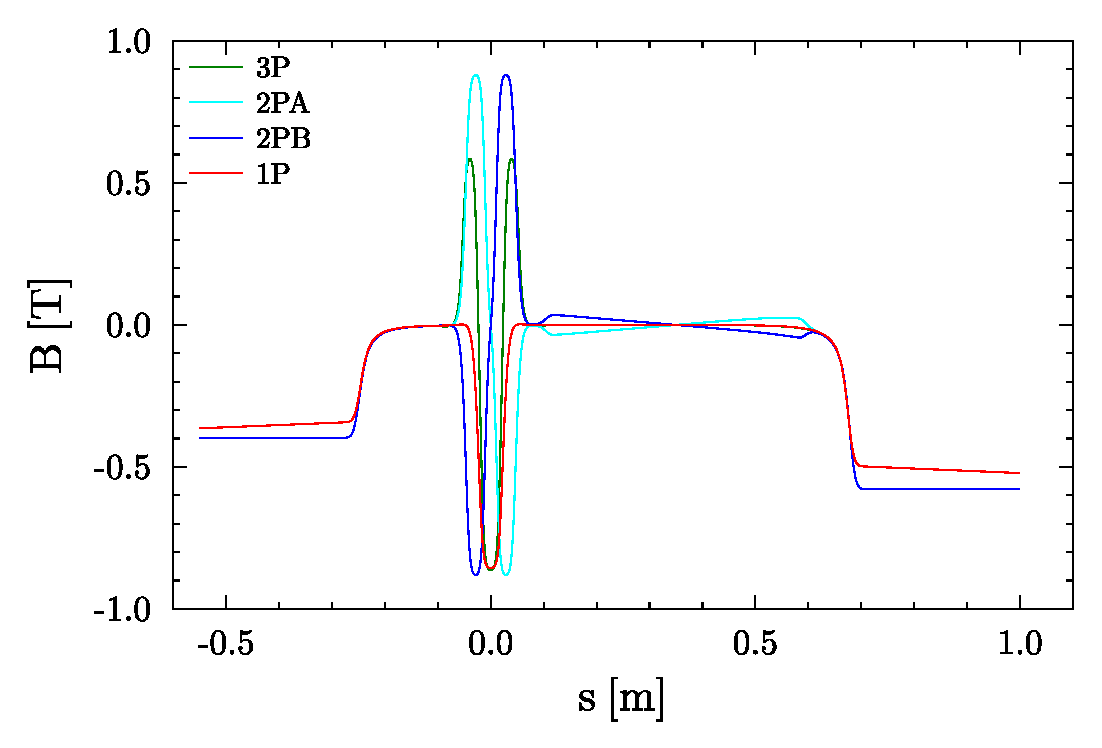
\includegraphics[keepaspectratio,width=5in]{GRAPHICS/wiggler_field.eps}
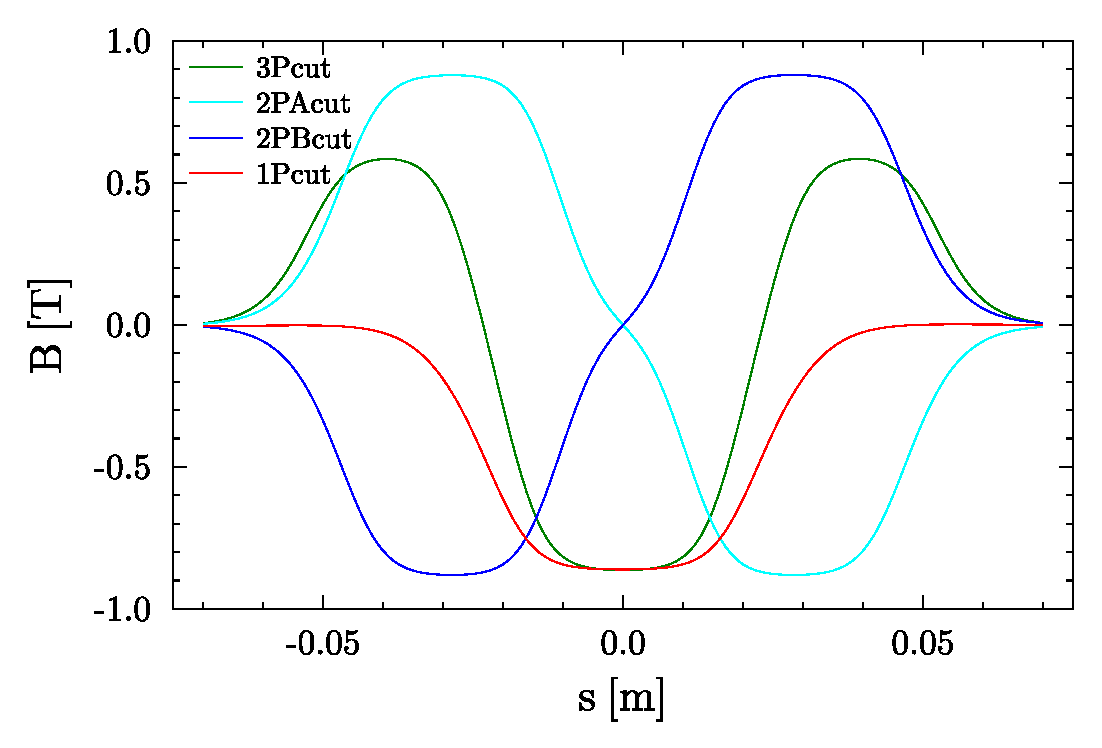
\includegraphics[keepaspectratio,width=5in]{GRAPHICS/wiggler_field_cut.eps}
\caption{a) (Top) Magnetic field for the different short ID (data from Joel Chavanne). b) (Bottom) The same field data ``cut'' in a limited $s$ interval only showing the
field produced by the short ID's.} 
\end{figure}


\section{Radiation spectrum}
The full emission spectrum produced by the IDs with magnetic field in Fig.~\ref{figurewigglerfield}b is compared with 
a the $0.856~T$ bending magnet (integrated over $2~mrad$ horizontal divergence) in Fig.~\ref{figurespectra}. It can be shown that 
the 1P spectrum is very similar to the current BM spectrum (over $2~mrad$ horizontal divergence), The 2P is the most favorable case
(both A and B configurations present the same emission spectrum because full emission is considered and magnetic field is the 
same except for a sign). The 3P is more intense than the BM at low photon energies, and practically the same at high energies.
Table~\ref{tableflux} contains flux values for the photon energies studied here.



\begin{table}[H]
\label{tableflux}
\caption{Some values of flux.}
\vspace{0.3cm}
\begin{tabular}{cccccc}      % Alignment for each cell: l=left, c=center, r=right
\hline
Device    & 5 keV  & 10 keV  &  20 keV  & 40 keV   & 80 keV  \\
\hline
\input{GRAPHICS/table_flux.txt}
\hline
\end{tabular}
\end{table}



\begin{figure}[H]
\label{figurespectra}
\centering
%\includegraphics[width=1.0\textwidth]{spectra.eps}
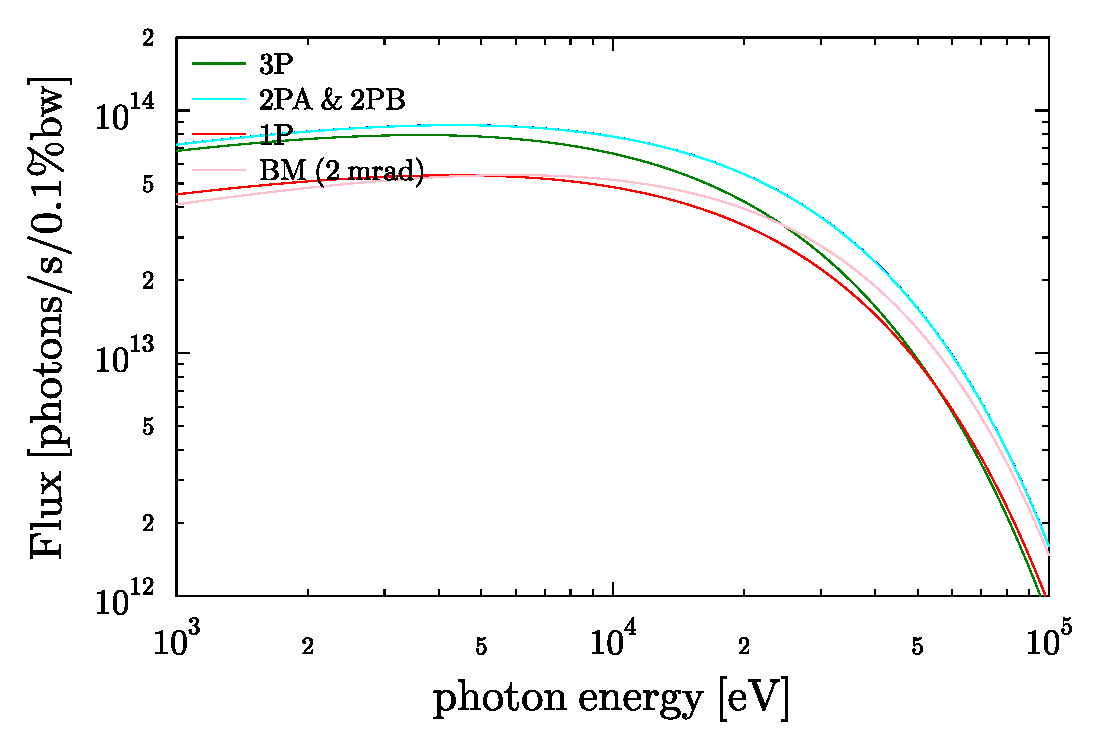
\includegraphics[keepaspectratio,width=5in]{GRAPHICS/spectrum.eps}
\caption{Calculated flux spectra produced by the ESRF-EBS short wigglers and the ESRF bending magnet.}
\end{figure}




\section{Radiation geometry}

In order to estimate the photon beam properties in the ideal case of {\it zero emittance} and no emission from the side BMs, 
a series of calculations have been preformed using the magnetic field in Fig.~\ref{figurewigglerfield}b. 
Results for all sources and focusing cases are summarized in Table~\ref{tabledivergenceszeroemittance}. 
Full results are in a supplement document {\tt short\_wigglers\_no\_emittance.html}. 
The calculations are performed for photon energy $E=5,~10,~20,~40,~80~keV$. 

Some comments about these results:
\begin{enumerate}
 \item the horizontal divergence is $< 2~mrad$. This is dictated by the maximum interval in transversal velocity which is approximately
 the maximum horizontal divergence $v_x/c \sim \theta_x$.
 \item the vertical divergence is dictated by the photon emission angle and decreases with photon energy.
 \item the ideal focus always presents tails due to the emission of different poles (for 2P and 3P) and the curved
 trajectory of the electrons (1P and BM). These tails are highly dependent on the geometry. These tails will be completetly smeared-out by
 the electron emittance (see later), because the FWHM values are usually very small. However, the tails for the 2PA and 2PB cases
 are higher than the half maximum, thus explaining the high values in these devices. 
 In fact, the 2P case is the less favorable because of the two identical sources are at the limit of resolution, but their distance contribute 
 to the width. In the other cases there is only one source (1P) or three (3P) but the central one dominates. 
 \item Even more pronounced, the toroidal 1:1 focusing shows small sizes for all cases, being the 2P the less favorable case as a result 
 of the separation between the two poles emission. For 3P the different pole emissions are also separated but the most intense central pole dominates.
 \item the focus of the short ID's is highly structured, because the emission is concentrated in the crests of the electron trajectory, 
and there is no emittance that smears out the source and the image. For this reason, the numeric values of FWHM in 
Table~\ref{tabledivergenceszeroemittance} may not be significative.
%  \item Technical consideration 1: Results for all IDs can be a bit better than presented as beamline is centered to the direction of electron entering
%  in the device (not in the middle of the device). However, this is not dramatic because the 1:1 ideal focusing is always good.
 \item Technical consideration: the intensity profiles sometimes shows some numerical artifacts: a lack of intensity (holes) at given position and
  perhaps this intensity moved to another position. This is due to a problem in the interpolation and spline routines and will be solved, but for the
  moment just keep in mind that this is a calculation problem and has not physical sense.


\end{enumerate}


\begin{table}[H]
\label{tabledivergenceszeroemittance}
\caption{Photon beam divergence for the different short ID's for zero emittance. 
Negative values: failed to compute FWHM (it useally happens when size is $\leq 1~\mu m$).
Mirrors have no slope errors. }
\vspace{0.3cm}
\begin{tabular}{cc|cc|cc|cc|cc}      % Alignment for each cell: l=left, c=center, r=right
\hline
E       & ID  & H Div     &  V Div     & H 1:1            &  V 1:1   & H 1:1    &  V 1:1   & H 3:1     &  V 3:1      \\
        &     &           &            & ideal            &  ideal   & toroid   &  toroid  & ellip     &  ellip  \\
$eV$    &     & $\mu rad$ &  $\mu rad$ & $\mu m$          &  $\mu m$ & $\mu m$  &  $\mu m$ & $\mu m$   &  $\mu m$\\
\hline
% created by /users/srio/Oasys/OasysRun/SHORT_WIGGLERS/short_wigglers.py
\input{table1.txt}
\hline
\end{tabular}
\end{table}

\section{Electron emittance}

Emittance values for the EBS-ESRF lattice have been calculated using the AT package, with lattice file {\tt S28CINJ.mat}, and emittance 
values of $\epsilon_x = 134~pm$ and $\epsilon_z = 5~pm$ and energy dispersion $\sigma_{\delta} = 10^{-3}$. The short ID center is at the lattice
coordinate $s_w = 13.8379~m$. Close to the short ID position, we find the DQ2C dipole upstream, and the quadrupole QF8 and dipole 
DQ1D downstream. Table~\ref{magnets} shows the position and values for these devices. Table~\ref{tabletwiss} shows the Twiss parameters.
% 
\begin{table}[H]
\label{magnets}
\caption{Position of the center of the magnets referred to the cell's $s$ coordinate and to the center of the ID ($s_w$).} 
\vspace{0.3cm}
\begin{tabular}{ccccccc}      % Alignment for each cell: l=left, c=center, r=right
\hline
AT       & magnet       & $s$     & $s-s_w$   &  length       & angle          & Magnetic field \\
index    & name         & ($m$)   & ($m$)     &  ($m$)        & ($rad$)        & ($T$)          \\
\hline
63       & DQ2C\_2      & 13.3872 & -0.4507   & 0.4           & 0.0078         &  0.393         \\
         & short ID     & 13.8379 & 0         & $~\sim$ 0.14  &                &  $\sim 0.8 $   \\
68       & QF8D         & 14.4302 & 0.5923    & 0.4840        &                &                \\
70       & DQ1D         & 15.0342 & 1.1963    & 1.0280        & 0.0292         &  0.567         \\
\hline
\end{tabular}
\end{table}
% 
% 
\begin{table}[H]
\label{tabletwiss}
\caption{Twiss parameters at center of devices} 
\vspace{0.3cm}
\begin{tabular}{cccccccccc}      % Alignment for each cell: l=left, c=center, r=right
\hline
magnet   &  $s$      &  $\alpha_x$ & $\alpha_z$ & $\beta_x$ & $\beta_z$ & $\gamma_x$ &  $\gamma_z$ & $\eta_x$ & $\eta_z$ \\
name     &  ($m$)    &             &            & ($m$)     & ($m$)     & ($m^{-1}$) &  ($m^{-1}$) & $\eta_x$ & $\eta_z$ \\
\hline
% DQ2C\_2      &13.387  &  -0.584  &   1.364 &    0.605   &   4.421    &   2.216  &   0.647  &   0.012  &   0 \\
% short ID     &13.838  &  -2.018  &   1.933 &    1.814   &   2.569    &   2.797  &   1.844  &   0.018  &   0 \\
% QF8D         &14.430  &   2.618  &  -3.570 &    2.052   &   2.842    &   3.828  &   4.836  &   0.016  &   0 \\
% DQ1D         &15.034  &   0.128  &  -0.098 &    0.546   &   6.057    &   1.862  &   0.167  &   0.006  &   0 \\
% \hline
% created by /scisoft/users/srio/Working/rt/ESRF-new-lattice/REPORT-SHORT-WIGGLERS/GRAPHICS/ebs_find_fake_waist.py
\input{GRAPHICS/table_twiss.txt}
\hline

\end{tabular}
\end{table}
% 

At the ID center position the values of the $\alpha$ functions are large, meaning that the phase space ellipses at that position are tilted. 
The place where the phase ellipses are not tilted are called waist. At the waists, $\alpha = 0$ and the popular relation $\epsilon = \sigma \sigma'$
holds, where epsilon is the storage ring emittance (horizontal X, or vertical Z) and $\sigma$ and $\sigma'$ are related to the moments of the electron
distribution: $\sigma_x = <xx>^{1/2}$, $\sigma_x' = <x'x'>^{1/2}$ (and similarly for $y$). Outside the waist this relation does not hold (it can be
seen in Table~\ref{tablewaist} that for the ID center $\sigma_x \sigma_x' \simeq 587~pm > \epsilon_x$). Moreover, the electron size and divergences 
are dictated not only by the Twiss parameters but also by the energy dispersion (functions $\eta$, $\eta'$ and energy dispersion $\sigma_{\delta}$): 

\begin{eqnarray}
    <xx> = \beta_x \epsilon_x + \eta_x^2 \sigma_{\delta}^2 \cr
    <xx'> = - \alpha_x \epsilon_x + \eta_x \eta_x' \sigma_{\delta}^2 \cr
    <x'x'> = \gamma_x \epsilon_x + \eta_x'^2 \sigma_{\delta}^2 
\end{eqnarray}
and similarly for $y$. 

% Table~\ref{tablewaist} 
Table 6 gives the position of the waists closer to the ID center, and the electron beam sizes. 
% 
\begin{table}[H]
\label{tablewaist}
\caption{Values of $\alpha, \beta, \sigma$ and $\sigma'$ for position of the waists closer to the ID center. The values at the ID center 
are also shown. Relative positions means from ID to waist.
} 
\vspace{0.3cm}
\begin{tabular}{cccccccc}
\hline
location & waist $[m]$ &  waist $[m]$ &  $\alpha$    & $\beta$    & $\sigma$   & $\sigma'$ & $\sigma \sigma'$\\
         & (relative)  &  (absolute)  &              & $m$        & $\mu m$    & $\mu rad$ &     $pm$        \\
% \hline
% H upstream  ($\beta$ min)    &  {\bf -0.651}  &  13.187  &  -0.0007    &  0.491  &  {\bf 13.729}   & 16.524  \\
% H (center)                   &   0      &  13.838  &  -2.018018  &  1.814  &  23.766   & 19.358   \\
% H downstream ($\beta$ max)   &   0.327  &  14.165  &   0.0005    &  2.831  &  28.486   &  6.880   \\
% V upstream  ($\beta$ max)    &  -0.651  &  13.187  &   0.0003    &  4.700  &   4.848   &  1.031   \\
% V (center)                   &   0      &  13.838  &   1.9328    &  2.569  &   3.584   &  3.036   \\
% V downstream  ($\beta$ min)  &   {\bf 0.2855} &  14.123  &   0.0000    &  1.878  &   {\bf 3.64}   & 1.632   \\
\hline
% created by /scisoft/users/srio/Working/rt/ESRF-new-lattice/REPORT-SHORT-WIGGLERS/GRAPHICS/ebs_find_fake_waist.py
\input{GRAPHICS/table_waists.txt}
\hline     
\end{tabular}
\end{table}
% 

SHADOW include the effect of emittance. It asks for the values of the electron beam sizes and divergences {\bf at the waist} and the distance
from the waist. Then SHADOW calculates the values at any $s$ point along the ID by propagating these values {\bf in absence of magnetic field}.
In a typical case where the ID is placed in a long straight section, one should give to SHADOW the parameters at the waist, as indicated in 
Table~\ref{tablewaist}. However, in our case, the ID is very close to other magnets and the ``real'' waist positions are affected by these magnets, 
so the approximation of propagation in space absent of magnetic field is not valid. 

In order to give parameters to SHADOW, we can find the positions of ``fake'' waists corresponding to the location of waist supposing that the ID is
not surrounded by other magnets, but free space (no magnetic field). 
Fig.~3
%\ref{figfakewaist} 
shows the evolution of the cross 
terms $<xx'>$ and $<yy'>$ that are zero at the waists (also corrected by dispersion). From here, it can be found the ``fake'' horizontal 
waist at $s_w = -0.894~m$ and ``fake'' vertical waist at $s_w = 1.048~m$ from the ID center. Table~\ref{tablefakewaist} shows the values to be entered
to SHADOW for the fake waists and a comparison of the ``real'' and ``propagated'' values at the center of the ID, showing a good agreement. 



\begin{figure}[H]
\label{figfakewaist}
\centering
%\includegraphics[width=1.0\textwidth]{spectra.eps}
% created by /users/srio/Oasys/OasysRun/SHORT_WIGGLERS/ebs_find_fake_waist.py
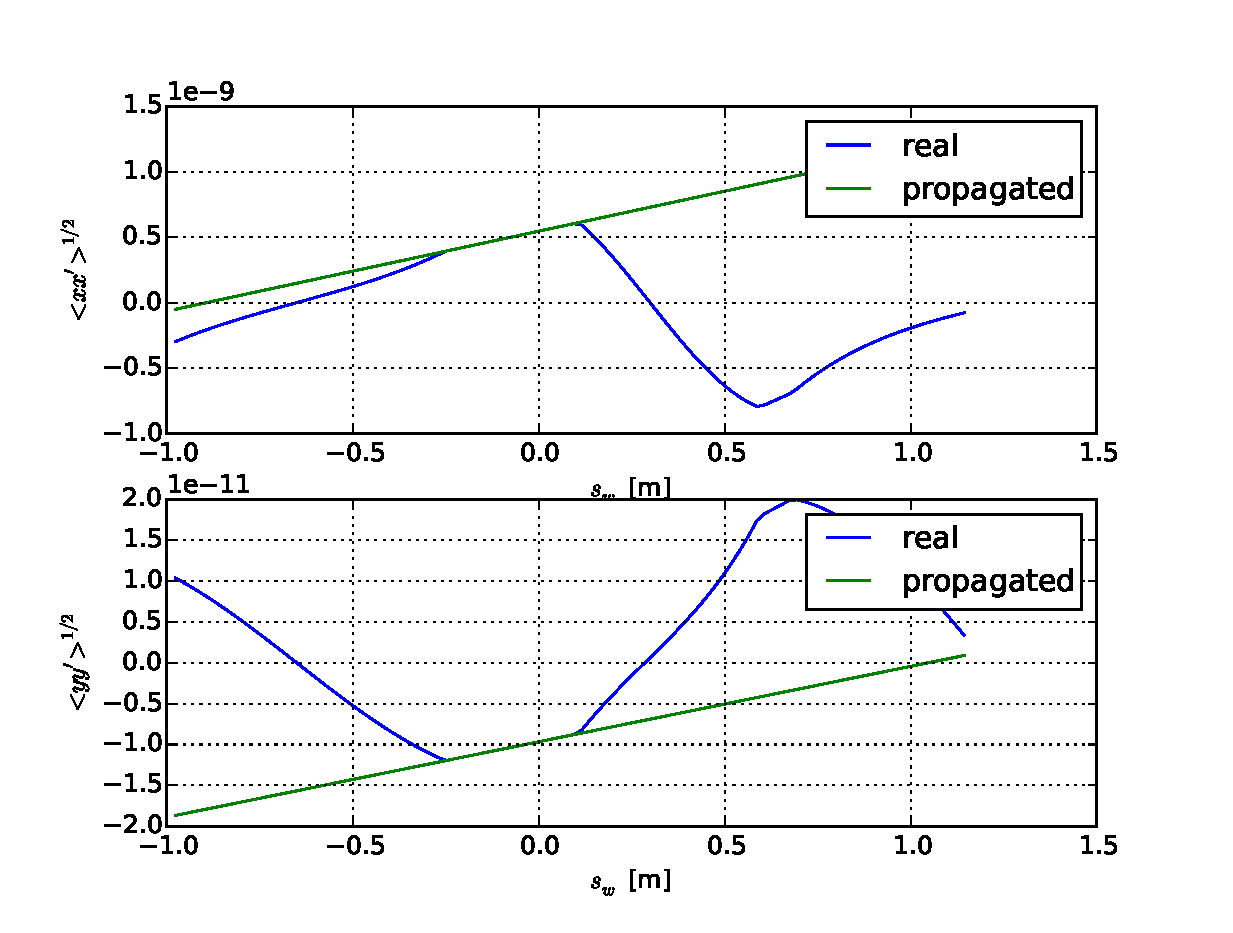
\includegraphics[keepaspectratio,width=5in]{GRAPHICS/fakewaists.eps}
\caption{Evolution of $<xx>^{1/2}$ and $<yy'>^{1/2}$ around the ID center, in the EBS-ESRF lattice (blue) and in absence of 
sourrounding magnets (green).}
\end{figure}



\begin{table}[H]
\label{tablefakewaist}
\caption{Values of the fake waists from where the propagation in absence of magnetic field gives correct values of electron beam 
moments at the ID center. 
Note that SHADOW input requires the distance from the waist to the ID center, thus the opposite
of the values given here. Also, the emittance value to be entered in SHADOW are $\sigma \sigma' $, (because dispersion is not considered in SHADOW). } 
\vspace{0.3cm}
\begin{tabular}{ccccc}
\hline
location                 & position   $[m]$ &  $\sigma$   & $\sigma'$ & $\sigma \sigma'$\\
                         & (relative)       &  $\mu m$    & $\mu rad$ &     $pm$        \\
\hline
H fake waist (downstream)&  -0.894         &  8.757      & 24.72     & 216.47      \\
H (center,propagated)    &   0             &  23.77      & 24.72     &             \\
H (center,real)          &   0             &  23.77      & 24.72     &             \\
\hline
V (center,real)          &   0             &  3.58       & 3.04      &             \\
V (center,propagated)    &   0             &  3.58       & 3.05      &             \\
V fake waist (upstream)  &  1.0480         &  1.647      & 3.036     & 5.00        \\
\hline 
\end{tabular}
\end{table}
% 

Figure~4
%\ref{figscatter} 
shows a sampling of the electron horizontal phase space at the center of the ID. 

\begin{figure}[H]
\label{figscatter}
\centering
%\includegraphics[width=1.0\textwidth]{spectra.eps}
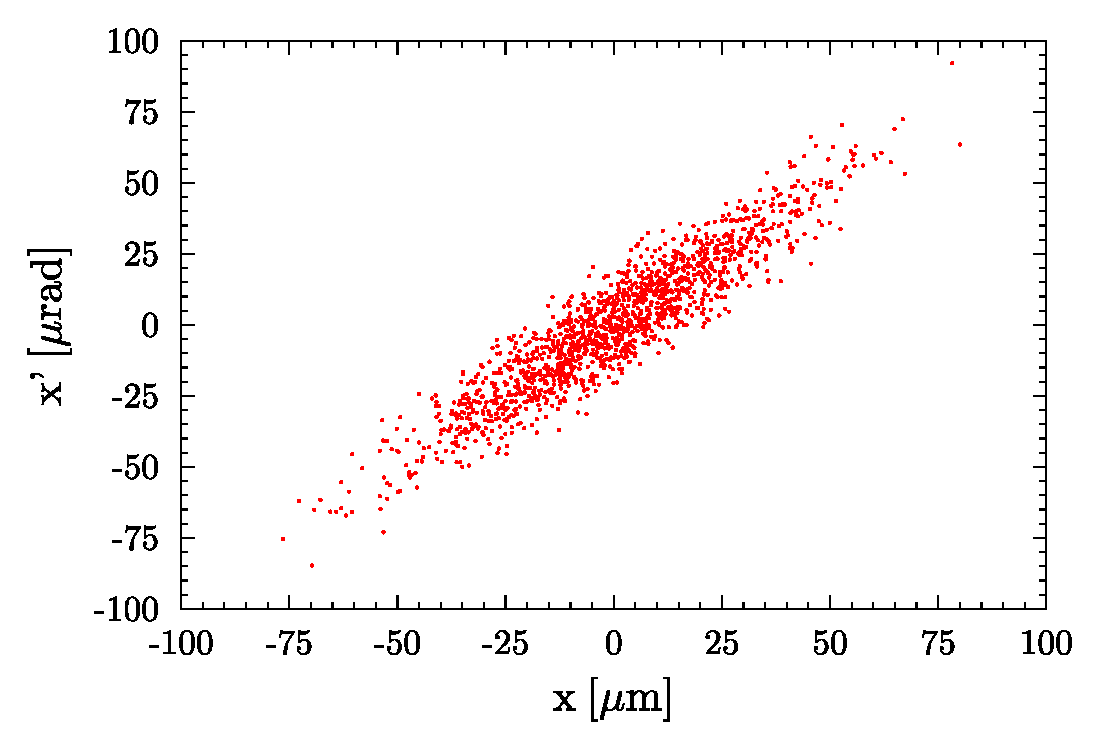
\includegraphics[keepaspectratio,width=5in]{GRAPHICS/scatter.eps}
\caption{Sampling of the electron  $(x,x')$ phase space at the center of the ID. }
\end{figure}


For the ESRF-I bending magnet the parameters used are taken from the Orange book ($\sigma_x = 77.9~\mu m , \sigma_x'= 110.9~\mu rad, 
\sigma_z = 12.9~\mu m, \sigma_z' = 0.5~\mu rad$) giving therefore  $\epsilon_x = \sigma_x \sigma_x' \sim 8600~pm $ and   
$\epsilon_z = \sigma_z \sigma_z' \sim 6.45~pm $. The distance to the waist has been taken to zero.
% 
The Table~\ref{tabledivergenceswithemittance} shows the results for the wigglers with field in Fig.~\ref{figurewigglerfield}b, but 
including emittance. Full results are in the file: {\tt short\_wigglers\_with\_emittance.html}. Some conclusions can be extracted:
\begin{enumerate}
 \item The divergence width values roughly vary as stated before (slightly reducing with photon energy in H and dictated by the photon emission in V)
 \item The 3P H divergence presents a hole in the middle, more important for low photon energies, but still present at 80 keV. This was discussed
  in a previous document \cite{myoldreport}. Also discussed there, the radiation presents ripples at the edges (not shown here, as these 
  interference effects are not considered by SHADOW). 
 \item The ideal focusing gives for all short IDs much better smaller foci than the BM placed at ESRF-I, due to the much better emittance values for 
 the new lattice. {\bf Thus, source brillance increases a lot.} For example, at 20 keV the 1:1 ideally focused BM beam is 173x30$\mu m^2$ and for
 the 3P in the new lattice it is 51x9$\mu m^2$, therefore a gain factor $\sim 12$. For the other cases, the gain goes from 6 to 15. 
 \item Ideal focus give too nice profiles (very well defined intensity distributions) much better than the profiles obtained by a more
 realistic 1:1 toroidal focusing. 
 Therefore, the ideal focus results results are usually not realistic for a typical beamline.
 \item For the 3P the 1:1 focused beam with a toroid does not resolve the ``three sources''. 
 \item The toroidal forcused 2P beam neither resolves the two sources, if the beamline is well aligned tangent to the inflexion point of the electron
 beam trajectory. In the case that the beamline is aligned tangent to the electrons entering in the ID, the two sources are resolved. There is a highest
 sensibility of the beamline alignment for the 2P as compared with the other cases, due to the presence of two identical sources.  
 \item 3:1 focusing always present some structures due to the extended source. These structures are always present, even for the 1P and BM, 
 so they are not originated by the multiple sources. 
 The focal size for 2P is worse than 1P and 3P, because of the same intensity in the two sources which contribute to enlarge the width, 
 as seen in the non-emittance case. However, the results are still very good (consider also that the 2P source is more intense than 1P and 3P).

 
\end{enumerate}

% 
\begin{table}[H]
\label{tabledivergenceswithemittance}
\caption{Photon beam divergence for the different short ID's for finite electron beam (with emittance). The toroidal and 
ellipsoidal mirrors have slope error of 0.85 $mu rad$ in the tangential direction. 
}
\vspace{0.3cm}
\begin{tabular}{cc|cc|cc|cc|cc}      % Alignment for each cell: l=left, c=center, r=right
\hline
E       & ID  & H Div     &  V Div     & H 1:1            &  V 1:1   & H 1:1    &  V 1:1   & H 3:1     &  V 3:1      \\
        &     &           &            & ideal            &  ideal   & toroid   &  toroid  & ellip     &  ellip  \\
$eV$    &     & $\mu rad$ &  $\mu rad$ & $\mu m$          &  $\mu m$ & $\mu m$  &  $\mu m$ & $\mu m$   &  $\mu m$\\
\hline
% created by /users/srio/Oasys/OasysRun/SHORT_WIGGLERS/short_wigglers.py
\input{table2.txt}
\hline
\end{tabular}
\end{table}
% 

\section{Overlapping radiation by the magnets in the neighbour}
For studing the overlapping effect of the side bending magnet, it is useful starting to study the effect of these BMs withouth insertion device. 
For that a case labelled ``0P'' (zero poles) is calculated for all cases studied here. Results are in the file: {\tt short\_wigglers\_with\_emittance.html}.
Looking at the intensity vesus divergence, it can be shown that for high photon energies the radiation from the downtream BM (DQ1D) dominates, because
its high magnetic field. This is not the case for low energies (e.g., at 5 keV), where the intensity of the emission from both BMs is similar. 
Moreover, at low energies the gap left between the radiation of the two BMs is very small, thus a background will be unavoidable. Ah high energies, the
separation gap increases, helping to isolate the ID radiation and reducing the background. In general, the size of the focused beam including theirside BMs
is similr to the size withouth BMs (compare in Table8 the values without BMs, labelled with ``cut'' with those with BMs). It can be concluded that a 
background from the side BMs is unavoidable, its effect is more important at low photon energies, and does not affect to the focal beam sizes. Because these
size beams are not focused at the same point than the central ID, their effect is less important when using focalization. However, each particular beamline
should be studied in more detail. 


\bibliography{report-short-wigglers-raytracing}
\end{document}
